\documentclass[11pt,a4paper]{article}

% --- Paquetes de Idioma y Tipografía ---
\usepackage[spanish, es-tabla]{babel}
\usepackage{fontspec}
\usepackage{unicode-math}
\usepackage{graphicx}

% --- Layout y Estética ---
\usepackage{amsmath}
\usepackage{booktabs}
\usepackage{geometry}
\usepackage[table]{xcolor} 
\usepackage{microtype}
\usepackage{siunitx}
\usepackage{fancyhdr}
\usepackage{titlesec}

% --- Definición de Colores ---
\definecolor{BLogicNavy}{HTML}{002E5D} 
\definecolor{IndustrialBlue}{HTML}{005EB8}
\definecolor{LightGray}{HTML}{E0E0E0}

% --- Configuración de Fuentes ---
\setmainfont{libertinusserif-regular.otf}[
    BoldFont = libertinusserif-bold.otf,
    ItalicFont = libertinusserif-italic.otf,
    BoldItalicFont = libertinusserif-bolditalic.otf
]
\setmathfont{STIXTwoMath-Regular.otf}
\setmonofont{lmmono10-regular.otf}

\geometry{top=3cm, bottom=3cm, left=2.5cm, right=2.5cm}

% --- Personalización de Títulos (Estética DIN-Minimal) ---
\titleformat{\section}
  {\color{BLogicNavy}\normalfont\Large\bfseries\scshape}
  {\thesection}{1em}{}[\titlerule]

\titleformat{\subsection}
  {\normalfont\large\bfseries}
  {\color{BLogicNavy}\textbullet\ \thesubsection}{1em}{}

% --- Definición de la Fase Actual ---
\newcommand{\faseactual}{MVP: Prototipado Iterativo} 

% --- Pie de Página Coherente con Portada ---
\pagestyle{fancy}
\fancyhf{}
\renewcommand{\headrulewidth}{0pt}
\renewcommand{\footrulewidth}{0.6pt} 

\fancyfoot[L]{\footnotesize \color{gray} \textbf{B-LOGIC NODES} $|$ \faseactual}
\fancyfoot[R]{\footnotesize \color{gray} Página \thepage}

% --- Metadatos y Protección Digital (CORREGIDO) ---
\usepackage[pdfauthor={Marcos Bernard Calixto Lopez},
            pdftitle={DomoNode - System Heartbeat Validation},
            pdfsubject={Ingeniería Electrónica - Capa 0},
            pdfkeywords={IoT, PIC16F1939, B-Logic Nodes},
            pdfstartview={FitH}, % Ajusta el zoom al ancho de la página al abrir
            colorlinks=true,
            linkcolor=BLogicNavy,
            urlcolor=IndustrialBlue]{hyperref}

\usepackage{pdfpages} % Para insertar páginas PDF completas

% --- Ruta de búsqueda para imágenes y PDFs ---
\graphicspath{{research/assets/}{assets/}}

\begin{document}

% --- PORTADA DIN-INDUSTRIAL CON PROTECCIÓN DE AUTOR ---
\begin{titlepage}
    \hrule height 2pt
    \vspace{0.4cm}
    
    \begin{flushleft}
        \begin{minipage}[t]{0.60\textwidth}
            {\color{BLogicNavy}\Large\addfontfeatures{LetterSpace=15}\textbf{B-LOGIC NODES}\par}
            \vspace{0.12cm}
            {\color{gray}\footnotesize\scshape IoT Node Framework | Hardware-to-Cloud Integration}
        \end{minipage}
        \begin{minipage}[t]{0.39\textwidth}
            \raggedleft
            {\color{gray}\scriptsize 
            \textbf{FASE} \ $|$ \ \faseactual \\ 
            \textbf{ITERACIÓN} \ $|$ \ 01}
        \end{minipage}
    \end{flushleft}
    
    \vspace{5.5cm}

    \begin{flushleft}
        {\color{gray}\footnotesize\scshape DomoNode Ecosystem}\par
        \vspace{0.25cm}
        {\Huge\addfontfeatures{LetterSpace=2}\textbf{System Heartbeat Validation}\par}
        \vspace{0.4cm}
        {\color{BLogicNavy}\hrule height 1.8pt width 11cm} 
        \vspace{0.6cm}
        {\small\textsf{Firmware Design \ $|$ \ Layer 0}}
    \end{flushleft}

    \vfill

    \begin{flushleft}
        \begin{minipage}{0.5\textwidth}
            \hrule width 3cm
            \vspace{0.3cm}
            {\footnotesize\color{gray}\scshape Responsable del Proyecto}\\
            \vspace{0.15cm}
            \textbf{Marcos Bernard Calixto López}\\
            {\small Ingeniería Electrónica}
        \end{minipage}
    \end{flushleft}

    \vspace{1.5cm}
    
    % Pie de página de la portada: Protección y Ubicación
    \hrule height 0.6pt
    \vspace{0.2cm}
    \begin{minipage}[t]{0.65\textwidth}
        {\color{gray}\tiny \textcopyright \ 2026 Marcos Bernard Calixto López. \\ Algunos derechos reservados. Licencia CC BY-NC-SA 4.0.}
    \end{minipage}
    \begin{minipage}[t]{0.34\textwidth}
        \raggedleft
        {\color{gray}\footnotesize Santiago de Surco, \today}
    \end{minipage}
\end{titlepage}

\newpage

% --- CUERPO DEL DOCUMENTO ---

\section{Comunicación: Requerimientos y Alcance}
Para el nodo \textbf{DomoNode}, se ha identificado la necesidad de una señal de diagnóstico de bajo nivel (\textit{Heartbeat}). El sistema requiere una validación visual inmediata tras un evento de \textit{Master Clear} (MCLR) que confirme la estabilidad del oscilador interno antes de iniciar procesos de mayor complejidad.

\section{Planificación Rápida}
En esta etapa del \textbf{\faseactual}, el sprint de diseño se centra en la \textbf{Capa 0 (Hardware Core)}, estableciendo los cimientos para las capas superiores del modelo OSI mediante los siguientes objetivos:
\begin{itemize}
    \item Selección de un pin de salida dedicado exclusivamente a diagnóstico visual.
    \item Configuración del oscilador interno (\texttt{INTOSC}) para minimizar el BOM (\textit{Bill of Materials}).
    \item Definición de una secuencia de inicio que diferencie el estado de arranque de la ejecución normal.
\end{itemize}

\section{Modelado y Diseño Rápido}
Diseño orientado al microcontrolador \textbf{PIC16F1939}. El enfoque iterativo permite definir constantes físicas reutilizables en versiones superiores.
Este diseño se estructura desde la configuración del silicio (\textbf{Capa 0}), garantizando que los registros fundamentales (Fuses y Clock Tree) operen dentro de los márgenes nominales antes de la ejecución del firmware de aplicación.

\subsection{Capa 0: Configuración de Base de Tiempo}
Se selecciona el bloque \textbf{MFINTOSC} a \SI{500}{\kilo\hertz}. El modelado de tiempos en el nivel de registros se rige por:
\begin{equation}
F_{CY} = \frac{F_{OSC}}{4} \implies \frac{\SI{500}{\kilo\hertz}}{4} = \SI{125}{\kilo\hertz} \implies T_{CY} = \SI{8}{\micro\second}
\end{equation}

\subsection{Capa Física: Asignación de Recursos (I/O Mapping)}
\begin{table}[h]
    \centering
    \caption{Especificaciones Técnicas de la Iteración 01}
    \vspace{0.3cm}
    \begin{tabular}{@{}llll@{}}
        \toprule
        \textbf{Recurso} & \textbf{Función} & \textbf{Capa} & \textbf{Pin / Valor} \\
        \midrule
        System Clock & Internal Oscillator & \textbf{0} (Register) & 0x68 (500kHz) \\
        Indicator LED & Heartbeat Status & \textbf{1} (Electrical) & RD7 (Pin 30) \\
        Reset Vector & MCLR Logic & \textbf{0} (Fuse) & Pin 1 (RE3) \\
        \bottomrule
    \end{tabular}
\end{table}

\subsection{Esquemático del Módulo de Validación}
Como se observa en la Figura \ref{fig:esquema_v1}, se implementa una etapa de potencia con un transistor NPN para el control del LED, desacoplo de alimentación y un nodo de reset físico mediante el pin MCLR[cite: 7, 30, 35].

\begin{figure}[!ht] % '!' fuerza la posición para evitar el salto de página
    \centering
    % trim= izquierda abajo derecha arriba, clip recorta el espacio sobrante
    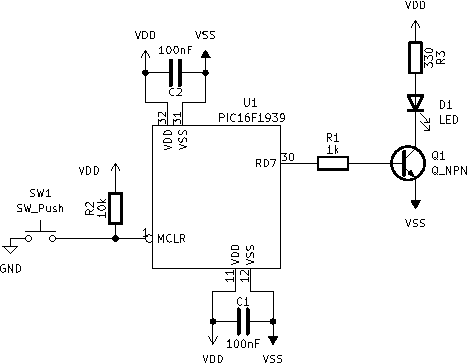
\includegraphics[width=0.7\textwidth, trim=0 0 0 0, clip]{DomoNode_V1_inkscape.pdf} 
    \caption{Diseño de hardware para la validación del System Heartbeat (Capa Física).}
    \label{fig:esquema_v1}
\end{figure}

% Eliminamos el \clearpage para que el texto de la Sección 4 suba

\section{Construcción del Prototipo}
Implementación física y carga de firmware.
\subsection{Montaje en Protoboard}
% Pendiente: Descripción del ensamblaje físico del PIC16F1939.
\subsection{Firmware (XC8)}
% Pendiente: Lógica de inicialización de registros y bucle principal.

\section{Despliegue y Entrega (Pruebas)}
Criterios de aceptación y validación del prototipo físico.
% Pendiente: Resultados de las pruebas de ráfaga y estabilidad.

\section{Retroalimentación (Feedback)}
Análisis de la iteración para mejora continua.
% Pendiente: Notas para la Iteración 02 (Diferencias simulación vs. realidad).

\end{document}